\documentclass[final]{beamer} % beamer 3.10: do NOT use option hyperref={pdfpagelabels=false} !
  %\documentclass[final,hyperref={pdfpagelabels=false}]{beamer} % beamer 3.07: get rid of beamer warnings
  \mode<presentation> { \usetheme{UFPoster} }
  \usepackage[english]{babel}
  \usepackage[latin1]{inputenc}
  \usepackage{amsmath,amsthm, amssymb, latexsym}
  %\usepackage{times}\usefonttheme{professionalfonts}  % times is obsolete
  \usefonttheme[onlymath]{serif}
  \boldmath
  \usepackage[orientation=portrait,size=a0,scale=1.4,debug]{beamerposter}                       % e.g. for DIN-A0 poster
  \title[Epi. on Emp. Nets]{Epidemics on Dynamic,\\ Empirical Networks}
  \author[Pearson \& Hladish]{Carl A.~B.~Pearson \&\ Thomas J.~Hladish}
  \institute[EPI-UF]{Emerging Pathogens Institute, University of Florida}
  \date{\today}
  
  \newcommand{\spacer}{\begin{column}{0.02\paperwidth}\end{column}}
  
\usepackage{Sweave}
\begin{document}
\input{poster-concordance}
  \begin{frame}{}
    \begin{columns}[t]
    \spacer{}
    \begin{column}[t]{0.33\paperwidth}
    \begin{block}{Introduction}
Contact networks are \textbf{intrinsically temporal}, but we often analyze them as \textbf{aggregated over time}.  This simplifies both analytical and simulation approaches, but with simulation approaches we may dis-aggregate with minimal additional complexity when we simulate on empirical networks.

We have a large population, multi-year dataset for geo-temporal co-location, based on anonymized access to a municipal WiFi system.  We use that data to explicitly consider compare the time evolution of network measures when aggregating on shorter time scales up to aggregating over the entire period.  We then use the network as a time-varying, empirical backbone for simulating infection spread.
%     \begin{block}{\large Fontsizes}
%       \centering
%       {\tiny tiny}\par
%       {\scriptsize scriptsize}\par
%       {\footnotesize footnotesize}\par
%       {\normalsize normalsize}\par
%       {\large large}\par
%       {\Large Large}\par
%       {\LARGE LARGE}\par
%       {\veryHuge veryHuge}\par
%       {\VeryHuge VeryHuge}\par
    \end{block}
    \begin{block}{Materials}
Should describe the data set here.  Collection times, number of data points, assorted other counts, etc.  Probably a table.  Links to source tools.
    \end{block}
    \begin{block}{Methods}
The network measures are derived in the standard way, with the edges aggregated on co-temporal, co-location within the varying windows. 

The epidemic simulation is based on conventional network Susceptible-Infectious-Recovered simulation.  We established the reference transmission probabilities by fitting to final sizes for typical influenza outbreaks in the associated city.

When simulating the epidemics, we randomly select an iniital infective.  Infectives are uniformly infectious for a period of days $\tau$, and while infectious spread the infection with transmission probability $p$ to each of their suspectible neighboors each day.  Who is in their neighboorhood, however, changes each day according to the empirical contact network.
    \end{block}
    \begin{block}{Mathematical Section}
Probably not relevant.  Maybe restate the network measures?  Diagram SIR flow?
    \end{block}
    \begin{block}{Conclusion}
The aggregation of empirical observations has important implications for simulation results.
    \end{block}
    \end{column}
    \spacer{}
    \begin{column}{0.6\paperwidth}
    \begin{block}{Results}
    \begin{figure}
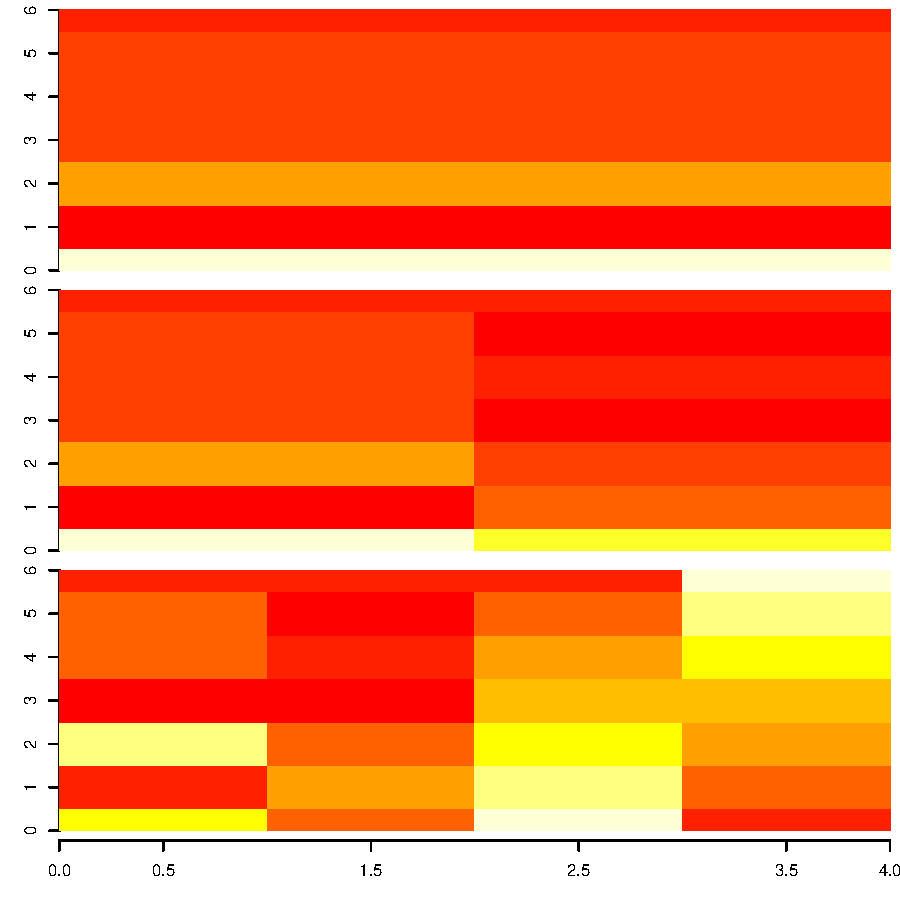
\includegraphics{poster-plotfig1}
%    
\includegraphics[width=0.8\linewidth]{placeholder.jpg}
    \caption{The first figure should be a series of comparisons of network measures (e.g., degree distribution) for the totally aggregated network vs averaged values of the network aggregated at different time periods - 1 year, 1 month, 1 week, 1 day.  May also want to do some heat charts of those measures through time, since the averages might hide neat insights like seasonality.}
    \end{figure}
    \begin{figure}
    
\includegraphics[width=0.8\linewidth]{placeholder.jpg}
    \caption{This should be the figure showing the simulation results for aggregation on whole network vs having day-by-day networks.  Probably should be two figures, one for final sizes and one for trajectories.  If we have time, multiples of these for some parameter variation.}
    \end{figure}
    
    \end{block}
    \vfill
    \end{column}
    \spacer{}
    \end{columns}
  \end{frame}
  \end{document}
 



% 
% 
% %----------------------------------------------------------------------------------------
% %	ADDITIONAL INFORMATION
% %----------------------------------------------------------------------------------------
% 
% \begin{block}{Additional Information}
% 
% Maecenas ultricies feugiat velit non mattis. Fusce tempus arcu id ligula varius dictum. 
% \begin{itemize}
% \item Curabitur pellentesque dignissim
% \item Eu facilisis est tempus quis
% \item Duis porta consequat lorem
% \end{itemize}
% 
% \end{block}
% 
% %----------------------------------------------------------------------------------------
% %	REFERENCES
% %----------------------------------------------------------------------------------------
% 
% \begin{block}{References}
% 
% \nocite{*} % Insert publications even if they are not cited in the poster
% \small{\bibliographystyle{unsrt}
% \bibliography{sample}\vspace{0.75in}}
% 
% \end{block}
% 
% %----------------------------------------------------------------------------------------
% %	ACKNOWLEDGEMENTS
% %----------------------------------------------------------------------------------------
% 
% \setbeamercolor{block title}{fg=red,bg=white} % Change the block title color
% 
% \begin{block}{Acknowledgements}
% 
% \small{\rmfamily{Thank the data source + ARO grant that's paying for CABP to attend.}} \\
% 
% \end{block}
% 
% %----------------------------------------------------------------------------------------
% %	CONTACT INFORMATION
% %----------------------------------------------------------------------------------------
% 
% \setbeamercolor{block alerted title}{fg=black,bg=norange} % Change the alert block title colors
% \setbeamercolor{block alerted body}{fg=black,bg=white} % Change the alert block body colors
% 
% \begin{alertblock}{Contact Information}
% 
% \begin{itemize}
% \item Web: \href{http://github.com/pearsonca/epidemics-4talk}{http://github.com/pearsonca/epidemics-4talk}
% \item Email: \href{mailto:cap10@ufl.edu}{cap10@ufl.edu}, \href{mailto:thladish@ufl.edu}{thladish@ufl.edu}
% \end{itemize}
% 
% \end{alertblock}
% 
% \begin{center}
% \begin{tabular}{ccc}
% 
\includegraphics[width=0.4\linewidth]{logo.png} & \hfill & 
\includegraphics[width=0.4\linewidth]{logo.png}
% \end{tabular}
% \end{center}
% 
% %----------------------------------------------------------------------------------------
% 
% \end{column} % End of the third column
% 
% \end{columns} % End of all the columns in the poster
% 
% \end{frame} % End of the enclosing frame
% 
% \end{document}
